%Szablon przygotowany przez mgr Marcina Hanca, z drobnymi zmianami dr Michała Rena
%Master's thesis - Decompiling Android OS applications by Dawid Drozd
\documentclass[12pt,a4paper,leqno,oneside,titlepage]{book}

% (TIP) Your editor should fit this line:
%%%%%%%%%%%%%%%%%%%%%%%%%%%%%%%%%%%%%%%%%%%%%%%%%%%%%%%%%%%%%%%

%%%%%%%%%%%%%%%%%%%%%%%%%%%%%%%%%%%%%%%%%%%%%%%%%%%%%%%%%%%%%%%
%%%%%%%%%%%%%%%%%%%%%%%%%%%%%%%%%%%%%%%%%%%%%%%%%%%%%%%%%%%%%%%
%                      config
%%%%%%%%%%%%%%%%%%%%%%%%%%%%%%%%%%%%%%%%%%%%%%%%%%%%%%%%%%%%%%%
%%%%%%%%%%%%%%%%%%%%%%%%%%%%%%%%%%%%%%%%%%%%%%%%%%%%%%%%%%%%%%%


% Wczytanie pakietów: kodowania, czcionki i języki.
\usepackage[utf8]{inputenc}
\usepackage{lmodern}
\usepackage[english,polish]{babel}
% Wczytanie pakietu 'polski' w celu zapewnienia polskich nazw.
\usepackage{polski}
% Czcionki matematyczne.
\usepackage{amsfonts}
\usepackage{amsmath}
% Floating images: https://tex.stackexchange.com/a/8633/139599
\usepackage{float}

% Ładne początki rozdziałów (pakiet fncychap).
% Polecam Sonny i Conny. Bjornstrup najładniejszy, ale mi się bugował.
\usepackage[Sonny]{fncychap}
% Ładne i klikalne odnośniki.
\usepackage{url}
% Odnośniki dla adresów z polskimi znakami.
\usepackage[]{hyperref}
% Możliwość tworzenia łączonych pól (wg. rzędów) w tabelach.
\usepackage{multirow}
% Pakiet do cytowania kodów źródłowych.
\usepackage{listings}
% Pakiet do ładnego wstawiania grafik.
\usepackage{graphicx}
% Pakiet dodający możliwość wstawienia rozdziału "Akronimy".
\usepackage{acronym}
% Pakiet dodający kolory
\usepackage[usenames,dvipsnames,svgnames,table]{xcolor}
% Pakiet rozwiązujący problem z underscore w Section.
\usepackage[T1]{fontenc}
% Pakiet dodający definicje i twierdzenia.
\usepackage{amsthm}

% Custom format of ARM Assembler source code
\usepackage{package/arm-assembler-latex-listings/lstlangarm}
% Custom format for JavaScript
\usepackage{package/lstlangjavascript}
% Custom format for Diff preview
\usepackage{package/lstlangdiff}

\frenchspacing

\newcommand{\myAuthorName}{Dawid Patryk Drozd}
\author{\myAuthorName{}}
\title{Dekompilacja aplikacji działających w systemie Android OS.}

% \imod{k} Ładny zapis dzielenia modulo.
\makeatletter
\def\imod#1{\allowbreak\mkern10mu({\operator@font mod}\,\,#1)}
\makeatother

% \rom{n} Liczba n zapisana rzymsko.
\makeatletter
\newcommand*{\rom}[1]{\expandafter\@slowromancap\romannumeral #1@}
\makeatother

% Własne definicje.
% \begin{mydef}
%     Treść definicji.
% \end{mydef}
\newtheorem{mydef}{Definicja}

% Ładny sposób wstawiania cytatu rozpoczynającego rozdział.
% \begin{chapquote}{KTO}
%     CO ONA POWIEDZIAŁA?
% \end{chapquote}
\makeatletter
\renewcommand{\@chapapp}{}
\newenvironment{chapquote}[2][2em]
  {\setlength{\@tempdima}{#1}%
   \def\chapquote@author{#2}%
   \parshape 1 \@tempdima \dimexpr\textwidth-2\@tempdima\relax%
   \itshape}
  {\par\normalfont\hfill--\ \chapquote@author\hspace*{\@tempdima}\par\bigskip}
\makeatother

% Zmiana tekstów w listingach kodów źródłowych na j. polski.
\renewcommand\lstlistingname{Kod źródłowy}
\renewcommand\lstlistlistingname{Spis kodów źródłowych}

% Redefinicja Abstract'ów.
% W celu możliwości wstawienia dwóch na jedną stronę.
\newenvironment{abstractpage}
  {\cleardoublepage\vspace*{\fill}\thispagestyle{empty}}
  {\vfill\cleardoublepage}
\newenvironment{abstract}[1]
  {\bigskip\selectlanguage{#1}%
   \begin{center}\bfseries\abstractname\end{center}}
  {\par\bigskip}

% Dodatkowe definicje stylu stron.
\lstset{
  basicstyle={\small\ttfamily},
  breaklines=true,
  columns=flexible,
  frame=single
}

% ToDo marker command
\newcommand{\todo}[1]{\colorbox{yellow}{#1}}

\setlength{\oddsidemargin}{0.5in}
\setlength{\textwidth}{5.7in}
\setlength{\topmargin}{0in}
\setlength{\textheight}{8.5in}
\linespread{1.05}

%%%%%%%%%%%%%%%%%%%%%%%%%%%%%%%%%%%%%%%%%%%%%%%%%%%%%%%%%%%%%%%
%%%%%%%%%%%%%%%%%%%%%%%%%%%%%%%%%%%%%%%%%%%%%%%%%%%%%%%%%%%%%%%
%                      begin{document}
%%%%%%%%%%%%%%%%%%%%%%%%%%%%%%%%%%%%%%%%%%%%%%%%%%%%%%%%%%%%%%%
%%%%%%%%%%%%%%%%%%%%%%%%%%%%%%%%%%%%%%%%%%%%%%%%%%%%%%%%%%%%%%%

% Tu rozpoczyna się zawartość pracy!
\begin{document}

% Strona tytułowa zgodna z wymaganiami:
% http://www.wmi.amu.edu.pl/pl/prace-dyplomowe
\begin{titlepage}
\let\footnotesize\small
\let\footnoterule\relax
\let \footnote \thanks

\begin{center}
{\large \bf Uniwersytet im. Adama Mickiewicza w Poznaniu \\ Wydział Matematyki i~Informatyki \par}
\vspace{0.5cm plus 1mm minus 2mm}
{{\bf Kierunek: Informatyka} \par}
\end{center}%

\vspace{1.5cm plus 1fill}
\begin{flushleft}
{\center {\bf \Large \myAuthorName{}} \\ \normalsize Nr albumu: \bf 362617\par}
\end{flushleft}
\vspace{1.5cm plus 1mm minus 2mm}

\begin{center}
{\huge\textbf{Dekompilacja aplikacji działających w systemie Android~OS}\par}
\vspace{0.5cm plus 1mm minus 2mm}
{\large Decompiling Android OS applications}
\par
\vspace{1.5cm plus 1.5fill}

\begin{flushright}\large
\begin{tabular}{l}
Praca magisterska\\[3pt]
\MakeUppercase{ }\\[3pt]
Promotor: \\[3pt]
\bfseries dr Michał Ren \\[3pt]
\end{tabular}
\end{flushright}
\vspace{4cm plus .1fill}
{\large 2017\par}
\end{center}
\end{titlepage}

% Zgłoszenie braku numerowania kolejnych stron.
\pagenumbering{gobble}

\begin{flushright}{
Poznań, dnia 25 czerwca 2017
}\end{flushright}
\begin{center}{
\par
\vspace{1.5cm plus 1.5fill}
{\large OŚWIADCZENIE}
}\end{center}
\par
\vspace{1.5cm plus 1.5fill}
Ja, niżej podpisany, \myAuthorName{}, student Wydziału Matematyki i~Informatyki Uniwersytetu im. Adama Mickiewicza w Poznaniu oświadczam, że przedkładaną pracę dyplomową pt.: ``Dekompilacja aplikacji działających w systemie Android OS'' napisałem samodzielnie. Oznacza to, że przy pisaniu pracy, poza niezbędnymi konsultacjami, nie korzystałem z pomocy innych osób, a~w~szczególności nie zlecałem opracowania rozprawy lub jej części innym osobom, ani nie odpisywałem tej rozprawy lub jej części od innych osób.\\

Oświadczam również, że egzemplarz pracy dyplomowej w~wersji drukowanej jest całkowicie zgodny z~egzemplarzem pracy dyplomowej w~wersji elektronicznej.\\

Jednocześnie przyjmuję do wiadomości, że przypisanie sobie, w~pracy dyplomowej, autorstwa istotnego fragmentu lub innych elementów cudzego utworu lub ustalenia naukowego stanowi podstawę  stwierdzenia  nieważności postępowania w~sprawie nadania tytułu zawodowego.\\

Wyrażam zgodę na udostępnianie mojej pracy w czytelni Archiwum UAM.\\

Wyrażam zgodę na udostępnianie mojej pracy w zakresie koniecznym do ochrony mojego prawa do autorstwa lub praw osób trzecich.
\par
\vspace{1.5cm plus 1.5fill}
\begin{center}{
..............................................\\
{\footnotesize(czytelny podpis studenta)}
}\end{center}


%%%%%%%%%%%%%%%%%%%%%%%%%%%%%%%%%%%%%%%%%%%%%%%%%%%%%%%%%%%%%%%
%%%%%%%%%%%%%%%%%%%%%%%%%%%%%%%%%%%%%%%%%%%%%%%%%%%%%%%%%%%%%%%
%                      Thanks to...
%%%%%%%%%%%%%%%%%%%%%%%%%%%%%%%%%%%%%%%%%%%%%%%%%%%%%%%%%%%%%%%
%%%%%%%%%%%%%%%%%%%%%%%%%%%%%%%%%%%%%%%%%%%%%%%%%%%%%%%%%%%%%%%

\newpage

\phantom{.}

\vspace{12cm} \hspace{1cm}\phantom{.}\\
\phantom{.}\hspace{5cm}{Składam serdeczne podziękowania}\\
\phantom{.}\hspace{5cm}{doktorowi}\\
\phantom{.}\hspace{5cm}{Michałowi Renowi}\\
\phantom{.}\hspace{5cm}{za jego nieocenioną pomoc}\\
\phantom{.}\hspace{5cm}{przy pisaniu tej pracy.}\\
\phantom{.}\hspace{5cm}{}\\
\phantom{.}\hspace{5cm}{Dziękuję również}\\
\phantom{.}\hspace{5cm}{Małgorzacie Cabaj}\\
\phantom{.}\hspace{5cm}{za wsparcie gramatyczne}\\
\phantom{.}\hspace{5cm}{przy pisaniu tej pracy.}\\


%%%%%%%%%%%%%%%%%%%%%%%%%%%%%%%%%%%%%%%%%%%%%%%%%%%%%%%%%%%%%%%
%%%%%%%%%%%%%%%%%%%%%%%%%%%%%%%%%%%%%%%%%%%%%%%%%%%%%%%%%%%%%%%
%                      Bookmarks
%%%%%%%%%%%%%%%%%%%%%%%%%%%%%%%%%%%%%%%%%%%%%%%%%%%%%%%%%%%%%%%
%%%%%%%%%%%%%%%%%%%%%%%%%%%%%%%%%%%%%%%%%%%%%%%%%%%%%%%%%%%%%%%

\newpage
% Przód pracy - spisy i abstrakty.
\frontmatter
% Spis treści ze specjalnym uwzględnieniem podkreśleń w tytułach sekcji.
\pagestyle{plain}
{
    \catcode`\_=12
    \tableofcontents
}
% Spis ilustracji.
\listoffigures
% Spis tabeli.
\listoftables
% Spis listingów kodów źródłowych.
\begingroup
\let\clearpage\relax
\lstlistoflistings
\endgroup

%%%%%%%%%%%%%%%%%%%%%%%%%%%%%%%%%%%%%%%%%%%%%%%%%%%%%%%%%%%%%%%
%%%%%%%%%%%%%%%%%%%%%%%%%%%%%%%%%%%%%%%%%%%%%%%%%%%%%%%%%%%%%%%
%                      Abstract
%%%%%%%%%%%%%%%%%%%%%%%%%%%%%%%%%%%%%%%%%%%%%%%%%%%%%%%%%%%%%%%
%%%%%%%%%%%%%%%%%%%%%%%%%%%%%%%%%%%%%%%%%%%%%%%%%%%%%%%%%%%%%%%

% Strona z abstraktami.
\begin{abstractpage}
% Abstrakt w języku polskim.
\begin{abstract}{polish}
Celem pracy jest omówienie procesu dekompilacji aplikacji mobilnych pisanych na system operacyjny Android.
Na początku poznamy budowę aplikacji androidowej. Korzystając z tej wiedzy nauczymy się obsługi narzędzi, które ułatwiają proces dekompilacji. Dzięki tym narzędziom otrzymamy wynik deasemblacji i nauczymy się go interpretować. Z tak otrzymanego wyniku postaramy się poskładać wszystko z powrotem do działającej aplikacji. Dowiemy się także jak system Android identyfikuje i weryfikuje pochodzenie aplikacji. Na koniec dowiemy się jakie niebezpieczeństwo niesie za sobą źle zabezpieczony kod aplikacji. Prześledzimy również proces, który utrudnia odzyskiwanie kodu źródłowego za pomocą technik odwrotnej inżynierii.
 
\end{abstract}
\smallskip
\noindent \textbf{Słowa~kluczowe:} RE, reverse engineering, inżynieria odwrotna, dekompilacja, android, apk, apktool, smali, zaciemnianie kodu,  deasembler, disassembler, objdump, asembler, dekompilator, release, debug, dex, hash, C++, Java

%Abstrakt w języku angielskim.
\begin{abstract}{english}
\todo{translate when PL is done}
\end{abstract}
\smallskip
\noindent \textbf{Keywords:} \todo{translate when PL is done}
\end{abstractpage}

% Finally - PRACA!
\mainmatter

%%%%%%%%%%%%%%%%%%%%%%%%%%%%%%%%%%%%%%%%%%%%%%%%%%%%%%%%%%%%%%%
%%%%%%%%%%%%%%%%%%%%%%%%%%%%%%%%%%%%%%%%%%%%%%%%%%%%%%%%%%%%%%%
%                      Introduction
%%%%%%%%%%%%%%%%%%%%%%%%%%%%%%%%%%%%%%%%%%%%%%%%%%%%%%%%%%%%%%%
%%%%%%%%%%%%%%%%%%%%%%%%%%%%%%%%%%%%%%%%%%%%%%%%%%%%%%%%%%%%%%%

% Wstęp jest uwzględniony w spisie treści jako rozdział bez numeru.
\addcontentsline{toc}{chapter}{Wstęp}
\chapter*{Wstęp}

Inżynieria wsteczna (ang. \emph{reverse engineering}, w skrócie RE) jest procesem analizy budowy i sposobu działania oprogramowania. Proces ten często jest długim procesem ze względu na to, że analizujemy kod który poprzednio został przekształcony przez inne programy (kompilatory, preprocesory, itp.) do formy mniej czytelnej. Takim przykładem może być skompilowany program napisany w C++.


\lstinputlisting[language=C++, captionpos=b, belowcaptionskip=4pt, caption={Przykładowy program w C++.}]{src/sample.cpp}

 

\lstinputlisting[language={[ARM]Assembler}, captionpos=b, belowcaptionskip=4pt, caption={Uproszczony kod po odwrotnej inżynierii dla platformy ARM.}]{src/sample.s}

Przykład, choć krótki, już pokazuje jak mamy utrudnione zadanie. Często analizujemy kod, który jest bardziej zrozumiały dla maszyny niż człowieka.

Proces inżynierii wstecznej jest dodatkowo utrudniany przez programistów, którzy nie chcą by ktoś podglądał jak pewna funkcjonalność została zrealizowana. W tym celu stosowane jest zaciemnianie kodu. Jednakże, inżynieria wsteczna czasem jest jedynym sposobem na dowiedzenie się, jak coś działa. Przykładem może być zarówno brak kodu źródłowego pewnej biblioteki, jak i brak dokumentacji do niej. Innym przykładem może być chęć dodania lub naprawienia pewnej funkcjonalności. Producent mógł porzucić rozwój oprogramowania, a nasza organizacja z pewnych powodów nie może zmienić tej biblioteki.

Celem tej pracy jest przedstawienie narzędzi i procesu dekompilacji zbudowanych aplikacji oraz ponownej kompilacji zmodyfikowanej aplikacji na system operacyjny Android.

\chapter{Jak zbudowana jest aplikacja na Android'a}
% https://en.wikipedia.org/wiki/Android_application_package
\section{Format .apk}

Rozszerzenie nazwy pliku bierze się z \emph{Android Package Kit (APK)}.
Format pliku przypomina ten znany z plików .jar
Pliki oznaczone tym rozszerzeniem służą do rozpowszechniania aplikacji na system android. Na skład paczki .apk wchodzą:

\begin{itemize}
\item skompilowany kod Java w formacie .dex
\item zasoby takie jak .png czy .mp3
\item certyfikaty
\item plik manifestu
\end{itemize}
Nazwa pliku jest dowolna pod warunkiem, że jest zakończona przez .apk
Pliki APK są pewnego rodzaju archiwum, które bazuje na formacie ZIP.
\begin{figure}[H]
	\centering
	\includegraphics[height=0.3\textheight]{img/apk_content_as_zip.png}
	\caption{Otworzony plik .apk za pomocą programu ark}
\end{figure}
Szczegółowa budowa paczki apk:
\begin{itemize}
\item \texttt{Katalog META\_INF}
\begin{figure}[H]
	\centering
	\includegraphics[height=0.3\textheight]{img/apk_content_as_zip_meta_inf.png}
	\caption{META INF w ark}
\end{figure}
W katalogu znajduje się plik MANIFEST.MF. Plik ten zawiera metadane dotyczące zawartości paczki:\\\\
Przykład:
\begin{lstlisting}
Manifest-Version: 1.0
Built-By: Generated-by-ADT
Created-By: Android Gradle 2.3.3

Name: res/drawable-hdpi-v4/abc_list_longpressed_holo.9.png
SHA1-Digest: KQunCQh0E4bP0utgN0cHdQr9OwA=

Name: res/drawable-xxhdpi-v4/abc_ic_star_half_black_16dp.png
SHA1-Digest: EikVyBT5I7pmbJO2k8qF0V5hUc0=

Name: res/drawable-hdpi-v4/com_facebook_tooltip_black_background.9.png
SHA1-Digest: +DxTpyUKpT11iz68MG1Q0iB2EvA=

Name: res/drawable/common_google_signin_btn_icon_dark_normal.xml
SHA1-Digest: Qa00to2cn7JphS3q33GWp3lxTUs=
\end{lstlisting}

\item CERT.RSA - certyfikat aplikacji
\item CERT.SF
Lista zasobów i ich SHA-1. Skład jest taki sam jak w przypadku MANIFEST.MF


\item Folder lib
Katalog opcjonalny, w którym powinny znajdować się skompilowane biblioteki natywne na daną platformę np. armeabi, x86, mips

\item AndroidManifest.xml - dodatkowy plik manifestu, który zawiera między innymi nazwy, wersję i prawa aplikacji. Plik ten często jest binarnym XML, który łatwo zamienić na formę czytelną dla człowieka.

\item resources.arsc - plik zawierający prekompilowane zasoby takie jak binarne XML

\item folder assets
Folder zawierający zasoby, które nie są poddane dodatkowym obróbkom przez proces budowania apk.

\item folder res
Folder zawierający zasoby, które nie zostały przetworzone i dołączone do pliku resources.arsc

\item classes.dex Skompilowane pliki Java do formatu .dex, które rozumie Dalvik virtual machine

\end{itemize}


%https://en.wikipedia.org/wiki/Dalvik_(software)
%https://source.android.com/devices/tech/dalvik/dex-format

\section{Format .dex}

W pliku classes.dex są przechowywane definicje naszych klas i wszystkich innych danych im towarzyszących.
Format ten służy do przenoszenia danych wejściowych dla Dalvik Bytecode. 

Istnieją wymogi, które musi spełniać plik .dex, aby zostać uznany za prawidłowy.
% https://source.android.com/devices/tech/dalvik/constraints


W zapisie binarnym pliku na samym początku musi pojawić się tak zwany \verb|DEX_FILE_MAGIC|, który jest zdefiniowany w następujący sposób:
\begin{lstlisting}
ubyte[8] DEX_FILE_MAGIC = { 0x64 0x65 0x78 0x0a 0x30 0x33 0x38 0x00 }
                        = "dex\n038\0"
}
\end{lstlisting}
Jest on po to by mieć pewność, że odczytywany plik jest plikiem typu .dex.\\
W tym identyfikatorze jest zawarty znak nowej lini \verb|'\n' (0x0a)| i znak końca tekstu \verb|'\0' (0x00)|. Służy to tylko dodatkowym zabezpieczeniom, by wykryć uszkodzenie danych.
\\
Wartość ta zawiera także numer wersji formatu. Są to 3 cyfry pomiędzy nową linią a znakiem \verb|null|. Oczywiście służą w celach ewolucji danego formatu.
\\
Plik .dex jest podzielony na sekcje określone przez nagłówek.
\begin{itemize}
\item\verb|string_ids|  W tej sekcji znajdują się wszystkie identyfikatory dla wszystkich stringów w tym pliku. Lista tych stringów musi być posortowana po nazwie przy użyciu \verb|UTF-16|, nie uwzględniając ustawień lokalnych komputera. Lista jest unikatowa, czyli nie zawiera powtórzeń.
\item\verb|type_ids| Lista wszystkich typów występujących w pliku (zdefiniowanych i zadeklarowanych), tj. klasy, tablice, typy prymitywne. Lista ta jest posortowana po \verb|string_id| index i nie zawiera duplikatów.
\item\verb|proto_ids|	
Opis:
	Lista wszystkich prototypów metod znajdujących się w tym pliku.
Specyfika danych:
	Lista zawiera unikaty
	Lista jest posortowana po:
		typie zwracanym (jego indeksie w \verb|type_id|
		po liście argumentów i ich \verb|type_id|\\
Lista wszystkich prototypów metod znajdujących się w tym pliku. Lista jest posortowana. 
\item\verb|field_ids|
Opis:
	Lista wszystkich identyfikatorów pól.	
Specyfika danych:
	Lista jest posortowana po typie (jego indeksie \verb|type_id|), następnie po nazwie pola (jego indeksie \verb|string_id|)
	Lista nie zawiera duplikatów.	
\item\verb|method_ids|
Opis:
	Lista wszystkich identyfikatorów metod.
Specyfika danych:
	Lista nie zawiera duplikatów.
	Lista jest posortowana po definiowanym typie (jego indeksie \verb|type_id|),
	następnie po nazwie (jego indeksie \verb|string_id|) i na koniec po prototypie metody (jego indeksie \verb|proto_id|)

\end{itemize}
Rozszerzenie nazwy pliku bierze się z \emph{Android Package Kit (APK)}.
Format pliku przypomina ten znany z plików .jar
Pliki oznaczone tym rozszerzeniem służą do rozpowszechniania aplikacji na system android. Na skład paczki .apk wchodzą:

\begin{itemize}
\item skompilowany kod Java w formacie .dex
\item zasoby takie jak .png czy .mp3
\item certyfikaty
\item plik manifestu
\end{itemize}
Nazwa pliku jest dowolna pod warunkiem, że jest zakończona przez .apk
Pliki APK są pewnego rodzaju archiwum, które bazuje na formacie ZIP.

\begin{figure}[H]
	\centering
	\includegraphics[height=0.3\textheight]{img/apk_content_as_zip.png}
	\caption{Otwarty plik .apk za pomocą programu ark}
\end{figure}

Szczegółowa budowa paczki apk:
\begin{itemize}
\item \texttt{Katalog META\_INF}

\begin{figure}[H]
	\centering
	\includegraphics[height=0.3\textheight]{img/apk_content_as_zip_meta_inf.png}
	\caption{META INF w ark}
\end{figure}

W katalogu znajduje się plik MANIFEST.MF. Plik ten zawiera metadane dotyczące zawartości paczki:

Przykład:

\begin{lstlisting}
Manifest-Version: 1.0
Built-By: Generated-by-ADT
Created-By: Android Gradle 2.3.3

Name: res/drawable-hdpi-v4/abc_list_longpressed_holo.9.png
SHA1-Digest: KQunCQh0E4bP0utgN0cHdQr9OwA=

Name: res/drawable-xxhdpi-v4/abc_ic_star_half_black_16dp.png
SHA1-Digest: EikVyBT5I7pmbJO2k8qF0V5hUc0=

Name: res/drawable-hdpi-v4/com_facebook_tooltip_black_background.9.png
SHA1-Digest: +DxTpyUKpT11iz68MG1Q0iB2EvA=

Name: res/drawable/common_google_signin_btn_icon_dark_normal.xml
SHA1-Digest: Qa00to2cn7JphS3q33GWp3lxTUs=
\end{lstlisting}

\item CERT.RSA - certyfikat aplikacji
\item CERT.SF
Lista zasobów i ich SHA-1. Skład jest taki sam jak w przypadku MANIFEST.MF


\item Folder lib
Katalog opcjonalny, w którym powinny znajdować się skompilowane biblioteki natywne na daną platformę np. armeabi, x86, mips

\item AndroidManifest.xml - dodatkowy plik manifestu, który zawiera między innymi nazwy, wersję i prawa aplikacji. Plik ten często jest binarnym XML, który łatwo zamienić na formę czytelną dla człowieka.

\item resources.arsc - plik zawierający prekompilowane zasoby takie jak binarne XML.

\item folder assets
Folder zawierający zasoby, które nie są poddane dodatkowym obróbką przez proces budowania apk.

\item folder res
Folder zawierający zasoby, które nie zostały przetworzone i dołączone do pliku resources.arsc

\item classes.dex Skompilowane pliki Java do formatu .dex, które rozumie Dalvik virtual machine

\end{itemize}

\todo{Dokończyć tę sekcję}

\chapter{Narzędzia do dekompilacji}

\section{apktool}

Narzędzie to służy do przeprowadzenia odwrotnej inżynierii na wskazanym pliku apk. Potrafi zdekodować źródła aplikacji do formy zbliżonej przed jej zbudowaniem. Wiele procesów zostało zautomatyzowanych, takich jak zbudowanie ponowne aplikacji ze zdekompilowanych źródeł. \\
\lstinline|apktool| jest otwarto źródłowym oprogramowaniem na licencji \mbox{Apache 2.0 License.} \\
\\
Kod narzędzia jest dostępny na: \url{https://github.com/iBotPeaches/Apktool} \newline
Strona narzędzia: \url{https://ibotpeaches.github.io/Apktool/}
\newline
\newline
Aplikacja jest napisana w języku Java, dzięki czemu działa bezproblemowo na większości systemach operacyjnych. Jest to aplikacja bez interfejsu graficznego, aplikacja działa w konsoli.
\subsection{Dekompilacja}
Przykład użycia zostanie zaprezentowany na przykładowej aplikacji. Zakładając, że mamy już dostępne nasze \lstinline|.apk|\\
\begin{lstlisting}[language=bash]
{master} ~/Projects/UAM/
$ cd apktool
{master} ~/Projects/UAM/msc/apktool
$ ./apktool d ../sample-android-app/Thesis/app/app-release.apk 
I: Using Apktool 2.2.3 on app-release.apk
I: Loading resource table...
I: Decoding AndroidManifest.xml with resources...
I: Loading resource table from file: /home/gelldur/.local/share/apktool/framework/1.apk
I: Regular manifest package...
I: Decoding file-resources...
I: Decoding values */* XMLs...
I: Baksmaling classes.dex...
I: Copying assets and libs...
I: Copying unknown files...
I: Copying original files...
\end{lstlisting}
Dzięki tej komendzie uzyskamy źródła z naszej aplikacji. 
\begin{figure}[H]
	\centering
	\includegraphics[height=0.3\textheight]{img/apktool/sample_apk.png}
	\caption{Wynik pracy \lstinline|apktool d app-release.apk|}
\end{figure}
\begin{itemize}
\item{Folder \verb|smali|}\\
Zawiera odzyskane inżynierią wsteczną kody źródłowe naszej aplikacji. Kody jednak nie będą w języku Java, a w Smali. Smali jest omówiony w \ref{smali}.
\item{Folder \verb|original|}\\
Zawiera oryginalne źródła z naszego \verb|.apk| takie jak oryginalny \verb|AndroidManifest.xml| czy  \verb|META-INF|
\item{Folder \verb|lib|}\\
Zwiera natywne biblioteki wykorzystywane przez aplikację. W naszym przykładzie jest to skompilowana dynamiczna biblioteka z jedną prostą funkcją. Aby odzyskać kod natywny, musielibyśmy sięgnąć do innych narzędzi.
\item{Folder \verb|res|}\\
Zawiera wszystkie oryginalne zasoby naszej aplikacji, które zostały wcześniej przetworzone i w odpowiedni sposób upakowane.
\item{\verb|apktool.yml|}
Plik z metadanymi od apktool.
\item{\verb|AndroidManifest.xml|}\\
Zdekodowany \lstinline|AndroidManifest.xml|.
\end{itemize}
%
\begin{figure}[H]
	\centering
	\includegraphics[width=1\textwidth]
	{img/apktool/sample_diff_manifest.png}
	\caption{Diff między AndroidManifest.xml z źródeł a odzyskanym z pliku .apk}
\end{figure}
%
\subsection{Budowanie z powrotem}
Aplikację możemy zbudować ponownie z naszych zasobów. Przykład tego zastosowania znajduje się poniżej.

\begin{lstlisting}[language=bash]
{master} ~/Projects/UAM/msc/apktool
$ ./apktool b ./app-release/
I: Using Apktool 2.2.3
I: Checking whether sources has changed...
I: Smaling smali folder into classes.dex...
I: Checking whether resources has changed...
I: Building resources...
I: Copying libs... (/lib)
I: Building apk file...
I: Copying unknown files/dir...
\end{lstlisting}
W taki sposób otrzymamy znowu zbudowaną aplikację, jednak nie będzie ona podpisana tym samym kluczem. Jaki wpływ na aplikację ma podpisanie kluczem jest omówione w \ref{signing} rozdziale.

\section{dex2jar}
% https://github.com/pxb1988/dex2jar
Narzędzie to służy do przeprowadzenia odwrotnej inżynierii na pliku \lstinline|.dex|. Program jest troszkę mniej wygodny w porównaniu do apktool, ponieważ sami musimy wywołać odpowiednie skrypty i wydobyć to czego chcemy.

\begin{lstlisting}[language=bash]
{master} ~/Projects/UAM/msc
$ cd dex2jar/dex2jar-2.0
{master} ~/Projects/UAM/msc/dex2jar/dex2jar-2.0
$ ./d2j-dex2smali.sh ../../sample-android-app/Thesis/app/app-release.apk
baksmali ../../sample-android-app/Thesis/app/app-release.apk -> app-release-out
\end{lstlisting}
W taki sposób uzyskamy nasze zdekompilowane pliki \verb|.smali|. Narzędzie to umożliwia również odzyskanie plików \verb|.class|, które później mogą posłużyć do analizy przez inne programy np. \verb|JD-GUI|
%
\section{Inne}
Oczywiście narzędzi istnieje znacznie więcej. Ja w mojej pracy jednak skupiłem się na \verb|apktool| ze względów na przyjemne użytkowanie i duże społeczeństwo zebrane wokół tego narzędzia.\\
Jednym z narzędzi wartych zainteresowania może być \href{http://vaibhavpandey.com/apkstudio/}{apkstudio}. Narzędzie to działa we współpracy z \verb|apktool|, i daje nam łatwy edytor dla developera.\\
Kolejnym narzędziem graficznym wartym sprawdzenia jest \href{https://github.com/ajitsing/apkToJava}{apkToJava}.

%- Zabezpieczenia przed modyfikowaniem aplikacji (podpisywanie apki certyfikatem,nazwa package apki)

\chapter{Identyfikacja i weryfikowanie aplikacji}

W systemie Android możemy wydzielić dwa sposoby weryfikacji aplikacji. Sposoby te służą do identyfikacji aplikacji wśród wszystkich innych aplikacji zainstalowanych w systemie.

\section{Nazwa paczki}
Nazwa paczki aplikacji jest podstawowym sposobem na zidentyfikowanie aplikacji w całym systemie. Założenie jest proste: nazwa paczki aplikacji musi być unikatowa w skali systemu. Oznacza to, że nie możemy mieć jednocześnie wiele aplikacji o takiej samej nazwie paczki. Oczywiście, w sklepie z aplikacjami Google Play ta zasada również obowiązuje. Jednak w naszym systemie możemy mieć zupełnie inną aplikację niż ta, która znajduje się w sklepie, a będą miały taką samą nazwę paczki. Oczywiście, nie będziemy mogli zainstalować ze sklepu takiej aplikacji póki nie usuniemy poprzedniej najpierw z systemu.\\
Jest to bardzo prymitywna metoda identyfikacji, którą łatwo oszukać i podszyć się pod inną aplikację. Obrona przed tego typem oszustwa poruszymy w \ref{signing}. Dobrą praktyką i ogólnie przyjętą konwencją jest to aby nazwa paczki była odwróconą domeną. Tak samo jak to ma miejsce w zwykłym nazewnictwie paczek przy projektach w języku Java.
\begin{center}
	\centering	\includegraphics[height=0.3\textheight]
	{img/signing/google_play_app_name.png}
\end{center}
Na powyższym rysunku możemy zobaczyć nazwę paczki, która jest bezpośrednio widoczna w URL strony. Na tej też podstawie możemy dokonać wstępnej weryfikacji.
\begin{center}
	\includegraphics[height=0.3\textheight,keepaspectratio]
	{img/signing/two_same_aps.png}
\end{center}
Na powyższym rysunku możemy zobaczyć, że zostały zainstalowane dwie takie same aplikacje. Oczywiście zgodnie z zasadą, co służy do identyfikacji aplikacji jest nazwa paczki. W tym przypadku nazwa aplikacji i ikonka są takie same. Różnią się tylko nazwą paczki:
\begin{lstlisting}
com.f2zentertainment.pandemic
com.f2zentertainment.pandemic.qa
\end{lstlisting}
Podsumowując nazwa paczki służy tylko identyfikacji, tak jak w bazie danych \verb|ID| identyfikuje nam wiersz. 

\section{Cyfrowy podpis}
\label{signing}
% https://developer.android.com/studio/publish/app-signing.html
% https://source.android.com/security/apksigning/
% Różnica między certyfikatem a kluczem 
% https://pl.wikipedia.org/wiki/Certyfikat_klucza_publicznego
Wymogiem Android'a jest, by aplikacje były cyfrowo podpisane certyfikatem przed ich zainstalowaniem. Mamy dwa klucze publiczny i prywatny. Klucz publiczny jest dołączany do naszego \lstinline|.apk|. Dzięki temu w przyszłości będzie łatwo stwierdzić od kogo pochodzi nowa aplikacja czy aktualizacja. Narzędzie do podpisywania aplikacji (\lstinline|apksigner|) na Android'a pracuje na pliku \lstinline|.keystore|. Jest to binarny format, który zawiera jeden lub wiele prywatnych kluczy. 
\begin{figure}[H]
	\centering
	\includegraphics[width=1\textwidth,keepaspectratio]
	{img/signing/appsigning_selfmanagediagram_2x.png}
	\caption{Podpisanie aplikacji przez Developera.}
\end{figure}
Klucze są zabezpieczone dodatkowymi hasłami w pliku. Jeśli zgubimy lub utracimy nasz klucz to nie będziemy w stanie aktualizować naszej aplikacji użytkownikom. Jak wcześniej było wspomniane, aplikacja musi być podpisana tym samym kluczem, aby system uznał ją jako aktualizację, czy też autentyczną aplikację od danego twórcy.\par
Dekompilowane przez nas aplikacje możemy podpisać naszym kluczem co pozwoli nam na instalację tak zmodyfikowanej aplikacji. Jeśli jednak chcielibyśmy, aby system potraktował tak zmodyfikowaną aplikację jako aktualizację, to już się to nie powiedzie, ponieważ poprzednia aplikacja była podpisana innym kluczem.\par
Podpisana aplikacja służy jeszcze Androidowi do identyfikacji i tworzenia użytkowników, w których obrębie działa aplikacja. Aplikacje podpisane tym samym kluczem mają możliwość współdzielenia użytkownika, a co za tym idzie, aplikacje mogą współdzielić dane bez potrzeby tworzenia skomplikowanych interfejsów.\\
Android posiada dwa sposoby podpisywania aplikacji:\par
\begin{itemize}
\item{JAR signing (v1 scheme)}\par
Metoda ta bazuje na innej metodzie podpisywaniu pliku JAR. Pliki charakterystyczne dla tego sposoby podpisywania są plikami w katalogu \verb|META-INF| 
\par
\begin{figure}[H]
	\centering
	\includegraphics[width=1\textwidth,keepaspectratio]
	{img/signing/apk_signed_v1_vs_signed_with_v2.png}
	\caption{Przykładowy APK. Po lewej APK podpisany metodą v1, po prawej metodą v2}
\end{figure}
% https://source.android.com/security/apksigning/
% https://docs.oracle.com/javase/8/docs/technotes/guides/jar/jar.html#Signed_JAR_File
Wadą tej metody jest to, że nie chroni przed modyfikacjami pewnych obszarów APK, takich jak metadane. Dodatkowo program odpowiedzialny za weryfikację musi przetworzyć sporo danych, aby je zweryfikować. Takie podeście tworzy furtkę do ataku. Dodatkowo, trzeba odpakować wszystkie zasoby, co niestety jest też czasochłonne.
\item{APK Signature Scheme v2 (v2 scheme)}
Metoda ta dostępna jest od Android'a 7.0. Zawartość naszego APK przechodzi przez funkcję hashującą, której hash zostaje podpisany. Taki blok zostanie następnie dodany do naszego APK. Podczas walidacji, APK jest traktowane jako kontener i sprawdza hash'e wszystkich plików wewnątrz APK, łącznie z metadanymi. Nowy format jest kompatybilny wstecz. Starsze urządzenia zignorują dodatkowe dane i wykonają sprawdzanie według metody v1. Oczywiście, aplikacja musi być podpisana dwoma sposobami.
\end{itemize}
%
\begin{figure}[H]
	\centering
	\includegraphics[width=1\textwidth,keepaspectratio]
	{img/signing/apk-validation-process.png}
	\caption{Weryfikacja podpisu APK.}
\end{figure}
%
\chapter{Wynik deasemblacji}
%
\begin{figure}[H]
	\centering
	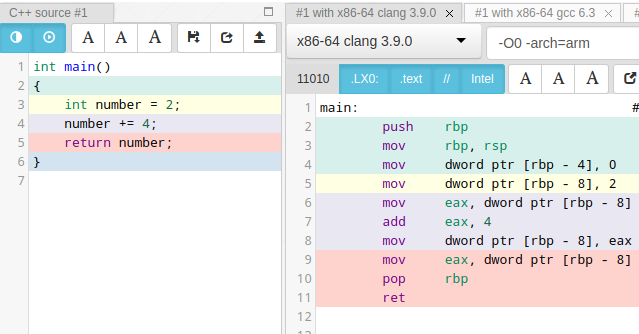
\includegraphics[height=0.3\textheight]{img/Screenshot_godbolt_org-sample.png}
	\caption{Wygenerowany przykład z strony \url{godbolt.org}}
\end{figure}

\section{SMALI}
\label{smali}
\todo{TODO}
\section{Dalvik/ART bytecode}
\todo{TODO}

\chapter{Sposoby ochrony przed deasemblacją}
% https://www.owasp.org/images/0/08/OWASP_SCP_Quick_Reference_Guide_v2.pdf
Naturalną odpowiedzią na atak, jest obrona. Mając takie proste w użyciu narzędzia do RE, naturalne jest, że powstały techniki utrudniające RE. Oczywiście, wykorzystano w tym kierunku wiedzę z innych technologi, gdzie ów problemy występują od dziesiątek lat. Temat jest na tyle szeroki, że poruszę tylko te sposoby które są powszechnie stosowane w tworzeniu aplikacji na Android'a i są stosunkowo tanie/proste do wdrożenia. Większą bazę wiedzy na temat zabezpieczenia kodu przez inżynierią odwrotną można znaleźć na stronie \hyperlink{https://www.owasp.org/index.php/OWASP_Reverse_Engineering_and_Code_Modification_Prevention_Project}{OWASP}.
% https://stackoverflow.com/questions/43601498/protect-android-app-from-reverse-engineering
% http://resources.infosecinstitute.com/android-hacking-and-security-part-18-introduction-to-reverse-engineering/
\section{Zaciemnianie kodu}
% https://pl.wikipedia.org/wiki/Zaciemnianie_kodu
Technika ta, często też nazywana potocznie kolorowaniem kodu, jest jedną z podstawowych technik \textbf{utrudniających} odzyskanie kodu. Technika ta polega na zamienianiu czytelnych dla programisty wyrażeń na wyrażenia krótkie i nieczytelne dla ludzi napisy, oczywiście z zachowaniem poprawności i zasad danego języka. Dlatego też technika ta nie modyfikuje zachowania kodu, a jedynie sprawia, że reprezentacja kodu staje się mniej czytelna dla ludzi. Napisałem, że jest to technika utrudniająca inżynierię wsteczną, a nie zapobiegającą, bo jej celem jest tylko utrudnienie odczytania kodu, przez co proces staje się bardziej czasochłonny. Oczywiście, mocno zdeterminowanego napastnika to nie zniechęci.\par
Jako przykład posłuży nam kod napisany w języku JavaScript, który poddamy zaciemnianiu. W języku Java byłoby to jeszcze bardziej przekształcone ze względu na transformację do kodu bajtowego.
%
\lstinputlisting[language=JavaScript, captionpos=b, belowcaptionskip=4pt, caption={Przykładowy program w JavaScript.}]{src/obfuscation_source.js}
%
\lstinputlisting[language=JavaScript, captionpos=b, belowcaptionskip=4pt, caption={Kod poddany zaciemnianiu w JavaScript.}]{src/after_obfuscation_source.js}
%
Oczywiście skuteczność jak i wymyślność naszego obfuskatora zależy od jego twórcy. Powyższy kod możemy jeszcze bardziej sprawić brzydszym.
%
\lstinputlisting[language=JavaScript, captionpos=b, belowcaptionskip=4pt, caption={Kod poddany zaciemnianiu w JavaScript.}]{src/after_obfuscation_2_source.js}
%
Powyższe przykłady kodów zostały poddane tylko transformacjom, które nie zmieniły sposobu działania. Robią dokładnie to samo, zostały tylko zapisane w innych formach, mianowicie w takich, które dla człowieka utrudniają znacząco zrozumienie jego działania.\\
Pokażę na przykładzie jak wygląda dekompilacja kodu napisanego w języku Java z zaciemnieniem i bez niego.
%
\lstinputlisting[language=Java, captionpos=b, belowcaptionskip=4pt, caption={Prosta implementacja listy w języku Java.}]{src/java_sample/SampleJavaCode.java}
%
Powyższy kod skompilujemy i otrzymamy pliki \lstinline|.class|.
%
\begin{figure}[H]
	\centering
	\includegraphics[height=0.3\textheight]
	{img/secure_desasembly/compiled_sample_java.png}
	\caption{Wygenerowane pliki za pomocą komendy: \lstinline|javac SampleJavaCode.java|}
\end{figure}
%
Najbardziej interesującym nas plikiem jest \lstinline|SampleJavaCode$ForwardListImplementation.class|, ponieważ jesteśmy ciekawi jak ktoś zaimplementował ów strukturę danych.  Załóżmy, że otrzymaliśmy aplikację od kolegi, który wszystko spakował w JAR'a. Po otwarciu JAR'a zobaczylibyśmy wszystkie te pliki, które widzimy na zdjęciu. Sama już nazwa nam wskazuje, gdzie mamy szukać implementacji. Ironią losu jest, że im lepszej jakości kod ktoś napisał i nie poddał go procesowi zaciemnienia, tym prościej atakującemu będzie znaleźć to, czego szuka. Oczywiście, plik \lstinline|.class| jest plikiem z kodem bajtowym i czytanie go nic nam nie da, dlatego musimy go najpierw zdekompilować. Dla uproszczenia procesu skorzystamy z dekompilatora online \hyperlink{http://www.javadecompilers.com/processing}{javadecompilers.com}.
%
\lstinputlisting[language=diff, captionpos=b, belowcaptionskip=4pt,
caption={Różnica między kodem źródłowym a kodem, który został odzyskany z dekompilacji. Uzyskane za pomocą komendy: \lstinline|diff -u SampleJavaCode.java SampleJavaCode_decompiled.java > SampleJavaCode_decompile.diff|}]
{src/java_sample/SampleJavaCode_decompile.diff}
%
Różnica wydaje się nieznacząca, a przynajmniej nie utrudnia nam za bardzo analizowania ów kodu. Jednak, jeśli nasz kod poddamy zaciemnieniu, to nasz przykładowy JAR zostanie zmodyfikowany i nawet dzięki temu zmniejszy się rozmiar JAR'a z 2.6 KB na 1.6 KB.
%
\begin{figure}[H]
	\centering
	\includegraphics[height=0.3\textheight]
	{img/secure_desasembly/sample_obfuscation.png}
	\caption{JAR przed zaciemnieniem i po, za pomocą narzędzia proguard.}
\end{figure}
%
JAR po poddaniu obfuskcaji pozmieniał nazwy plików, dlatego teraz znacznie ciężej znaleźć interesujący nas plik. Dodatkowo, zdekompilowany kod zmienił trochę hierarchię naszych struktur, co może dodatkowo utrudnić nam analizę.
%
\lstinputlisting[language=Java, captionpos=b, belowcaptionskip=4pt,
caption={Plik \lstinline|a.java|, czyli odpowiednik \lstinline|class SampleJavaCode|}]
{src/java_sample/decompiled_after_obfuscation/a.java}
%
%
\lstinputlisting[language=Java, captionpos=b, belowcaptionskip=4pt,
caption={Plik \lstinline|b.java|, czyli odpowiednik \lstinline|class ForwardListImplementation|}]
{src/java_sample/decompiled_after_obfuscation/b.java}
%
%
\lstinputlisting[language=Java, captionpos=b, belowcaptionskip=4pt,
caption={Plik \lstinline|c.java|, czyli odpowiednik \lstinline|class Node|}]
{src/java_sample/decompiled_after_obfuscation/c.java}
%
%
\lstinputlisting[language=Java, captionpos=b, belowcaptionskip=4pt,
caption={Plik \lstinline|d.java|, czyli odpowiednik \lstinline|interface List|}]
{src/java_sample/decompiled_after_obfuscation/d.java}
%
Kody zostały przeze mnie lekko zmodyfikowane. Poprawiłem formatowanie kodu, aby można było go łatwiej czytać. Skorzystałem z autoformatera kodu dostępnego w IDE Eclipse.
\section{Proguard}
% https://www.guardsquare.com/en/proguard
% https://www.guardsquare.com/en/proguard/manual/examples#application
% http://www.javadecompilers.com
% https://en.wikipedia.org/wiki/ProGuard_(software)
Progauard jest narzędziem, które potrafi zmniejszyć, zoptymalizować i zaciemnić kod w języku Java. Jest darmowym narzędziem na licencji \href{https://en.wikipedia.org/wiki/GNU_General_Public_License#Version_2}{GPL v2}. Potrafi zoptymalizować kod bajtowy np. poprzez usunięcie nie używanego kodu.
\par Proguard jest częścią narzędzi do budowania aplikacji na Android'a i domyślnie jest włączony dla aplikacji w trybie \verb|release|. Oczywiście, w naszym projekcie możemy skonfigurować to narzędzie za pomocą plików konfiguracyjnych tak, aby realizowało powierzone mu zadania np. zaciemniania kodu.\par
Wadą tego narzędzia, jak i zarazem powodem, dla którego developerzy je wyłączają, jest modyfikowanie stosu wywołań (ang. stack trace) przez zmiany nazw naszych metod czy klas.
%
\begin{lstlisting}[caption={Przykładowy wyjątek dla nie zaciemnionego kodu.}]
Exception in thread "main" java.lang.IndexOutOfBoundsException
        at SampleJavaCode$ForwardListImplementation.insert(SampleJavaCode.java:37)
        at Test.main(Test.java:6)
\end{lstlisting}
%
\begin{lstlisting}[caption={Przykładowy wyjątek dla kodu który został zaciemniony.}]
Exception in thread "main" java.lang.IndexOutOfBoundsException
        at b.a(Unknown Source)
        at TestObfuscated.main(TestObfuscated.java:6)
\end{lstlisting}
%
W powyższym przykładzie mamy dosyć małą głębokość wywołań, co nie utrudnia nam znacząco jego interpretacji. Jednak problem znacząco wzrasta im dłuższy mamy stos wywołań.\par
Jak już było wspomniane, możemy konfigurować proguarda tak, aby nie zaciemniał kodu. Jednakże, dla nas niekoniecznie jest to dobre rozwiązanie. Oczywiście, proguard rozwiązuje ten problem i wytwarza nam plik z mapowaniem starych identyfikatorów na nowe tak, byśmy mogli po naszej stronie w prawidłowy sposób odczytywać stos wywołań.
%
\lstinputlisting{src/java_sample/mapping.config}
%
\par
Jednakże, developer często musi sam sporo skonfigurować. Do tego dochodzą problemy z wywołaniami przez refleksję, czy wywołania natywnego kodu (Java Native Interface). Suma tych problemów często przewyższa zysk z zaciemnienia kodu i nikt nie chce poświęcać na to czasu.
\section{Natywny kod}
Często prostą i polecaną techniką jest ukrycie krytycznych części kodu w natywnym kodzie. Przykładem może być przepisany fragment kodu do C++. Dzięki temu, takiego kodu nie będzie mógł odczytać nowicjusz, który nauczył się używać apktool'a, czy innego tego typu narzędzia. W takim przypadku będzie potrzebna zarówno nisko poziomowa wiedza, jak i znajomość danej platformy.\par
Takie rozwiązanie ma jednak też i swoje wady. Developer, który będzie tego sposobu używał musi również wiedzieć jak to zaimplementować, aby nie wywołać tym sposobem nadmiarowej ilości błędów. Dochodzą do tego problemy związane z przekazywaniem danych między kodem napisanym w Javie a np. C/C++. Oczywiście wykorzystanie natywnego kodu komplikuje nam zaciemnianie kodu. Sposób ten jak i zaciemnienie jednak nie służą zabezpieczeniu naszego kodu, a tylko utrudnieniu napastnikowi odczytania i przeanalizowania naszej implementacji.
\section{Szyfrowanie}
% http://www.javaworld.com/article/2077342/core-java/cracking-java-byte-code-encryption.html?page=2
W poprzednich sekcjach były poruszone tylko utrudnienia jakie możemy wprowadzić w naszym programie, aby kod nie został odczytany. Kolejnym sposobem na znaczące utrudnienie odzyskania kodu byłoby szyfrowanie naszych plików. Dzięki temu aplikacja byłaby tylko odszyfrowana w czasie działania aplikacji. Oczywiście dla zwiększenia bezpieczeństwa klucz deszyfrujący może być dostarczany z zewnętrznego nośnika np. z serwera.
\par
Jednakże, ta technika też nie jest idealna. Jeśli ktoś będzie bardzo zawzięty i będzie miał dużo czasu, to też uda mu się ominąć to zabezpieczenie. Główną zmianą jaką developer musiałby wprowadzić, by wykorzystać ów metodę, jest napisanie własnego ClassLoader'a. Taka klasa wiedziałaby jak stworzyć instancje naszej klasy, aby móc z niej skorzystać. Oczywiście nie musimy szyfrować całej aplikacji a tylko części najbardziej wrażliwe, tak jak miało to miejsce z wykorzystaniem kodu natywnego.
%
\section{Inne}
Inne techniki często bazują na bezpośrednim ataku w narzędzia, których używa się do odwrotnej inżynierii.
\\
\todo{Opisać tutaj przykłady takich technik z przykładowym atakiem}
\todo{serio nie istnieją lepsze techniki ?}
%
\chapter{Niebezpieczeństwa źle zabezpieczonego kodu}
%- Zabezpieczenia / Niebezpieczeństwa. Np wstrzykiwanie w zapytania do serwera. (Ogólnie omówić czemu warto/trzeba zabezpieczyć kod przed dekompilacją)
% http://esec-lab.sogeti.com/static/publications/10-hitbkl-drm.pdf
Często developerzy nie myślą o skutkach, jakie niesie za sobą odwrotna inżynieria na ich aplikacjach. Często API serwisów internetowych nie jest zabezpieczone w żaden sposób. To właśnie z pomocą inżynierii wstecznej można uzyskać pełne REST'owe API danego serwisu.
\par
Jako przykładem posłużę się trzema aplikacjami, w których odwrotna inżynieria może nam dostarczyć wielu ciekawych informacji. W ich przypadku, włączenie zaciemniania kodu nie przyniosło zadowalających wyników. Jednakże, nie należy winić procesu samego w sobie, a zwykłe niedbalstwo ze strony programistów.
%
\section{Hasła bez zaciemniania}
% https://docs.google.com/presentation/d/1EI8cfZ5Vl5fiC03C5dogrM5GRHfcLTechk1OHBnAy6E/edit#slide=id.g10f8594d37_0_334
Aplikacja, która dostarcza nam oferty zniżkowe typu kupony i rabaty, dzięki którym możemy coś kupić. Pierwszym sposobem, by zagwarantować sobie dostęp do ogromnej ilości kuponów, byłoby wydobycie ich z API twórcy aplikacji. Możemy taki proces zautomatyzować, co powinno nam dostarczyć łatwy dostęp do kodów rabatowych. Wystarczy przy użyciu narzędzia np. \verb|wireshark| nasłuchać w sieci lokalnej, jakie metody API są odpytywane, i zreprodukować zapytania. Na szczęście, twórca aplikacji zabezpieczył się przez użycie hasła do API, które jest ukryte w zapytaniu HTTPS, więc nie możemy go w łatwy sposób wydobyć. Tutaj przychodzi nam na pomoc RE. Przy użyciu narzędzia apktool uzyskujemy kod, który nie jest zaciemniony. W łatwy sposób możemy zgadnąć, jak ktoś trzyma hasło w kodzie, o ile stosuje dobre praktyki programistyczne. W tym przypadku, jest to strzał w dziesiątkę. Wystarczy przeszukać kod pod frazą \verb|"password"|.
%
\begin{figure}[H]
	\centering
	\includegraphics[width=1\textwidth]
	{img/why_secure/find_password.png}
	\caption{Szukanie hasła w źródłach aplikacji.}
\end{figure}
%
Dzięki prostemu i szybkiemu przeszukaniu kodu, możemy zerknąć bezpośrednio do pliku, w którym znajduje się odpowiedź na nasze pytanie.
%
\begin{figure}[H]
	\centering
	\includegraphics[width=1\textwidth]
	{img/why_secure/password_in_smali.png}
	\caption{Ukryte hasło.}
\end{figure}
%
\section{Generator tokenów}
Aplikacje mobilne coraz częściej służą jako metoda podwójnego uwierzytelniania, czy też identyfikowania użytkownika, ponieważ ciężko jest, aby ktoś posiadał tysiąc komórek. Pewna firma, która prawdopodobnie miała dosyć automatycznych agentów, które rejestrowały się w serwisie i wykonywały pewne akcje, zdecydowała się wyłączyć uwierzytelnianie kodem na e-maila i zmusić użytkowników do korzystania z generatora tokenów z ich aplikacji.
%
\begin{figure}[H]
	\centering
	\includegraphics[height=0.3\textheight]
	{img/why_secure/steam_tokener.png}
	\caption{Generator tokenów w aplikacji.}
\end{figure}
%
Dlatego od teraz wszystkie boty musiałyby posiadać swoją instancję aplikacji, aby móc generować tokeny. Jednakże, znów wystarczyło wykorzystać inżynierię zwrotną, aby wydobyć algorytm, który był odpowiedzialny za generowanie tokenów. Oczywiście, w tym przypadku aplikacja była poddana zaciemnianiu i nie jest tak prosto znaleźć, gdzie był ukryty ten algorytm. Oczywiście, po żmudnej analizie nieczytelnego kodu i analizowaniu wykonywania udało się odnaleźć ów algorytm i go wyodrębnić do przyjaznej skryptowej postaci. Wystarczyło ów algorytm odpowiednio zainicjalizować i gotowe. Nie potrzebujemy do tego dedykowanej aplikacji.
%
\section{Blokady}
Aplikacje często posiadają blokady, czy pewne inne nieudogodnienia np. dla użytkowników, którzy mają odblokowane urządzenie (rooted device). W przypadku pewnej aplikacji, ta na samym starcie sprawdza, czy urządzenie jest zrootowane i jeśli tak, to kończy swoje działanie, uniemożliwiając korzystanie z niej. 
%
\begin{figure}[H]
	\centering
	\includegraphics[width=0.6\textwidth]
	{img/why_secure/device_rooted_message.png}
	\caption{Komunikat od aplikacji Starbucks.}
\end{figure}
%
Korzystając z RE możemy odzyskać kod ów aplikacji i usunąć sprawdzanie, dzięki czemu aplikacja będzie dla nas działać. Kod aplikacji został poddany zaciemnieniu przez co ciężko było znaleźć, gdzie jest sprawdzany ten warunek. Z pomocą przyszedł komunikat, który wyświetlał się nam na ekranie. Jeżeli wyszukamy ów tekst w plikach aplikacji, to znajdziemy początek nici po której dojdziemy do naszego kłębka. 
%
\begin{figure}[H]
	\centering
	\includegraphics[width=1\textwidth]
	{img/why_secure/search_for_message.png}
	\caption{Szukanie wiadomości prezentowanej przez aplikację}
\end{figure}
%
Dzięki prostemu wyszukaniu gdzie jest używany komunikat, jesteśmy w stanie precyzyjnie znaleźć miejsce naszej blokady i je wyłączyć.
%
\begin{figure}[H]
	\centering
	\includegraphics[width=1\textwidth,keepaspectratio]
	{img/why_secure/disable_block.png}
	\caption{Wyłączenie blokady sprawdzającej czy urządzenie jest zrootowane.}
\end{figure}
%
Tego typu blokady tyczą się również sprawdzania, czy użytkownik używa płatnej aplikacji oraz czy dana funkcjonalność powinna być odblokowana.

\chapter{Projekt}
\todo{Propozycje projektu}\\
\todo{1. Aplikacja do odbierania prawa dostępu do internetu innym aplikacja zainstalowanym na telefonie użytkownika}
\todo{2. Biblioteka do zabezpieczania fragmentów kodu przed RE wykorzystująca szyfrowanie}
\todo{3. TBC}

%\chapter{Bibliografia}
\newpage
% Dodanie wpisu Bibliografia do Spisu Treści.
\addcontentsline{toc}{chapter}{Bibliografia}
% Styl bibliografii: unsrt lub plain
\bibliographystyle{plain}
\bibliography{bibliografia}

%%%%%%%%%%%%%%%%%%%%%%%%%%%%%%%%%%%%%%%%%%%%%%%%%%%%%%%%%%%%%%%
%%%%%%%%%%%%%%%%%%%%%%%%%%%%%%%%%%%%%%%%%%%%%%%%%%%%%%%%%%%%%%%
%%%%%%%%%%%%%%%%%%%%%%%%%%%%%%%%%%%%%%%%%%%%%%%%%%%%%%%%%%%%%%%
%%%%%%%%%%%%%%%%%%%%%%%%%%%%%%%%%%%%%%%%%%%%%%%%%%%%%%%%%%%%%%%
%%%%%%%%%%%%%%%%%%%%%%%%%%%%%%%%%%%%%%%%%%%%%%%%%%%%%%%%%%%%%%%
%%%%%%%%%%%%%%%%%%%%%%%%%%%%%%%%%%%%%%%%%%%%%%%%%%%%%%%%%%%%%%%
%%%%%%%%%%%%%%%%%%%%%%%%%%%%%%%%%%%%%%%%%%%%%%%%%%%%%%%%%%%%%%%
%%%%%%%%%%%%%%%%%%%%%%%%%%%%%%%%%%%%%%%%%%%%%%%%%%%%%%%%%%%%%%%

% Spis akronimów użytych w pracy
\chapter*{Akronimy}
\begin{acronym}
\acro{KISS}{Keep It Simple Stupid}
\acro{RE}{reverse engineering}
\acro{IT}{Information Technology}
\acro{APK}{Android Package}
\end{acronym}
\end{document}
